



\documentclass[a4paper,12pt,spanish]{article}

\usepackage[utf8]{inputenc}


\usepackage{blindtext}
%\usepackage{microtype}
\usepackage{amsfonts, amsmath, amsthm, amssymb}
%\usepackage{fancyhdr}
%\usepackage{index}
%\usepackage{multicol}    

%\usepackage{booktabs}

\usepackage[T1]{fontenc}
\usepackage[utf8]{inputenc}
\usepackage{graphicx}
\usepackage[spanish,es-tabla]{babel}
\usepackage{url}
\usepackage{enumitem}

\usepackage[unicode=true, pdfusetitle,
bookmarks=true,bookmarksnumbered=false,bookmarksopen=false,
breaklinks=true,pdfborder={0 0 1},backref=false,colorlinks=false]
{hyperref}

\usepackage{listings}
\usepackage{longtable}


\usepackage{siunitx} %para el sistema internacional
\usepackage[export]{adjustbox}
\usepackage{booktabs} 
\usepackage{subcaption}

\usepackage{float}


\newcommand{\address}[1]{
	\par {\raggedright #1
		\vspace{1.4em}
		\noindent\par}
}

\usepackage[table,xcdraw]{xcolor}


\pagenumbering{gobble}
\include{noNumberPage}
\pagenumbering{arabic}
\setcounter{page}{27}

%tutorial de tablas latex: https://manualdelatex.com/tutoriales/tablas

\usepackage{multirow}

% \usepackage[table,xcdraw]{xcolor}


%Inicio del documento (hasta que se cierre con \end{document}
\begin{document}
	
	
	\title{ Espectrometría de Partículas Alfa y Beta. Absorción de Partículas Alfa}
	
	%\author{Adrián Rivero Fernández}
	\date{}
	
	\maketitle
	
	
	\section{Objetivos de la práctica}
	
	\vspace{\baselineskip}
	
	1. Estudiar el espectro $\alpha$ del Am$^{241}$\\
	
	2. Determinar el alcance de las partículas $\alpha$ en el aire, y obtener la curva del alcance.\\
	
	3. Estudiar el espectro $\beta$ del Sr$^{90}$.\\
	
	4. Calibrar las energías del espectro $\beta$.\\
	
	5. Estudiar la conversión interna del Cs$^{137}$\\
	
	
	\section{Determinación del ruido de fondo}
	
	Al tratar de tomar medidas del fondo de radiación, vemos que no llega fondo de radiación $\alpha$ ni $\beta$ al detector. Esto es debido a que la radiación no atraviesa las paredes del detector.
	
	
\begin{figure}[H]
	\centering
	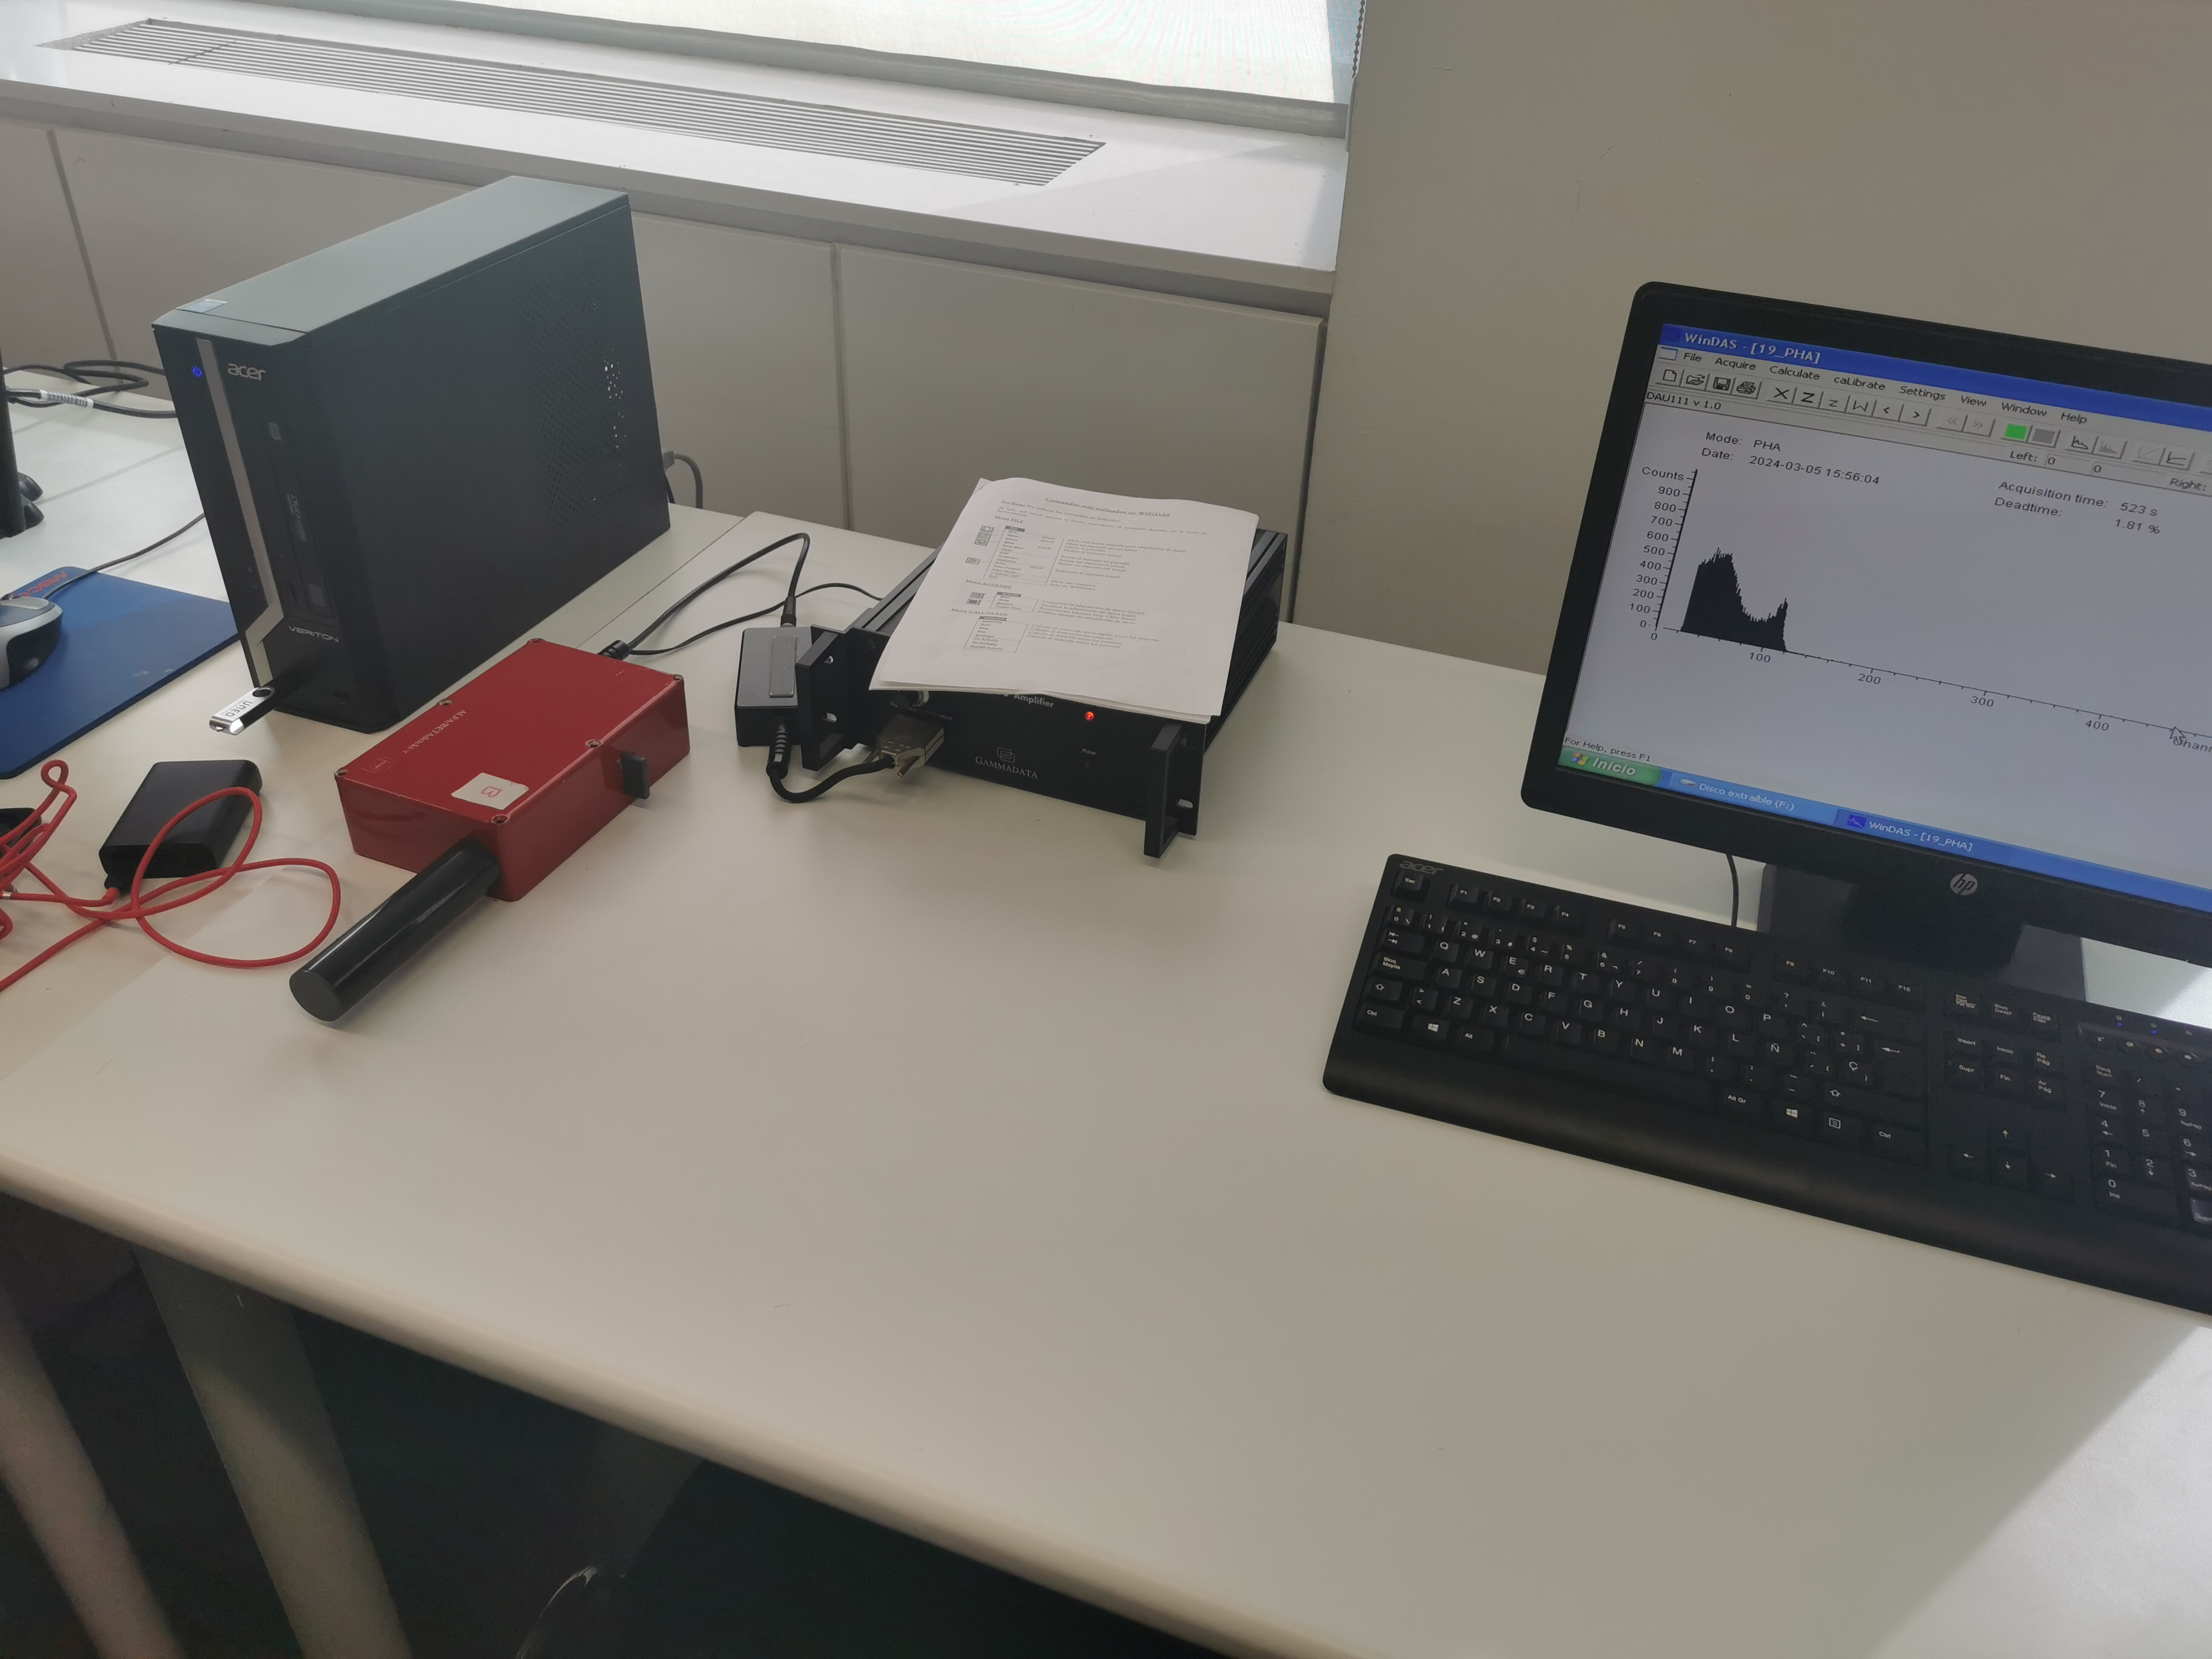
\includegraphics[width=0.7\linewidth]{imagenes/IMG_20240305_161034}
	\caption{Detector utilizado}
	\label{fig:img20240305161034}
\end{figure}
	
	\section{Espectro $\alpha$ del Am$^{241}$}
	
	A partir del esquema de desintegración del Americio-241, podemos ver que la distrubución de energía de la radiación tendrá una distribución con un pico en torno a 5,48MeV. 
	
	
	
\begin{figure}[H]
	\centering
	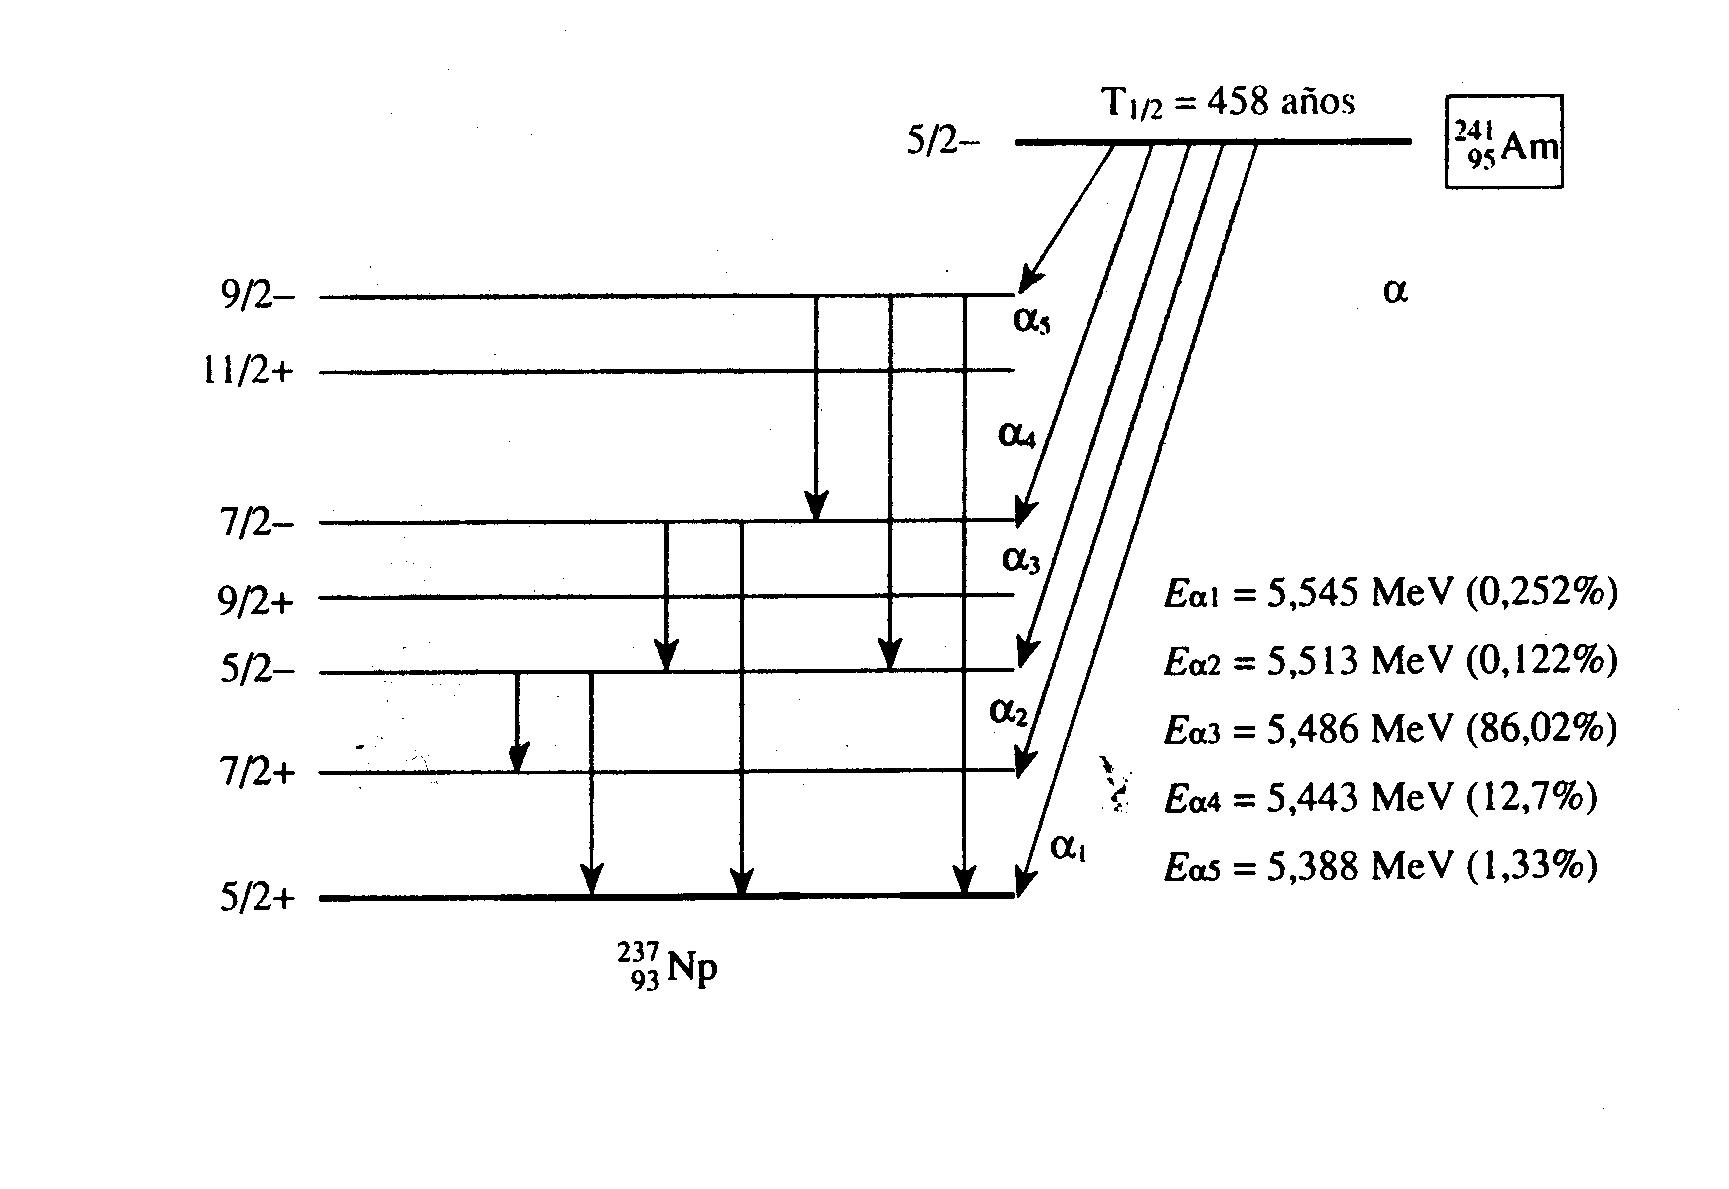
\includegraphics[width=0.7\linewidth]{imagenes/americio}
	\caption{Esquema de desintegración para el Am$^{241}$}
	\label{fig:americio}
\end{figure}
	
	
	
	
	Para distintas distancias de la muestra al detector, medimos el área del espectro acumulada durante 300 segundos.
	
	 
	 
	 \begin{figure}[H]
	 	
	 	\centering
	 	\begin{minipage}{0.45\textwidth}
	 		\centering
	 		\includegraphics[width=1.1\textwidth]{"graficas recortadas/11"} % first figure itself
	 		\caption*{Espectro para 1 cm}
	 	\end{minipage}\hfill
	 	\begin{minipage}{0.45\textwidth}
	 		\centering
	 		\includegraphics[width=1.1\textwidth]{"graficas recortadas/12"} % second figure itself
	 		\caption*{Espectro para 1,5 cm}
	 	\end{minipage}
 	
	 	\begin{minipage}{0.45\textwidth}
	 		\centering
	 		\includegraphics[width=1.1\textwidth]{"graficas recortadas/13"} % second figure itself
	 		\caption*{Espectro para 2 cm}
	 	\end{minipage}\hfill
	 	\begin{minipage}{0.45\textwidth}
	 		\centering
	 		\includegraphics[width=1.1\textwidth]{"graficas recortadas/14"} % second figure itself
	 		\caption*{Espectro para 2,5 cm}
	 	\end{minipage}
 	
		\begin{minipage}{0.45\textwidth}
		 	\centering
		 	\includegraphics[width=1.1\textwidth]{"graficas recortadas/15"} % second figure itself
		 	\caption*{Espectro para 3 cm}
		\end{minipage}\hfill
		\begin{minipage}{0.45\textwidth}
			\centering
			\includegraphics[width=1.1\textwidth]{"graficas recortadas/16"} % second figure itself
			\caption*{Espectro para 3,5 cm}
		\end{minipage}
	
	\caption{{Espectros del Am$^{241}$}}
	
	
	 \end{figure}
	 
	La baja resolución del detector y el ruido no permite distinguir los picos secundarios a distintas energías, una mayor resolución nos podría dar esa información. 
	
	
	
	\begin{figure}[H]
		\centering
		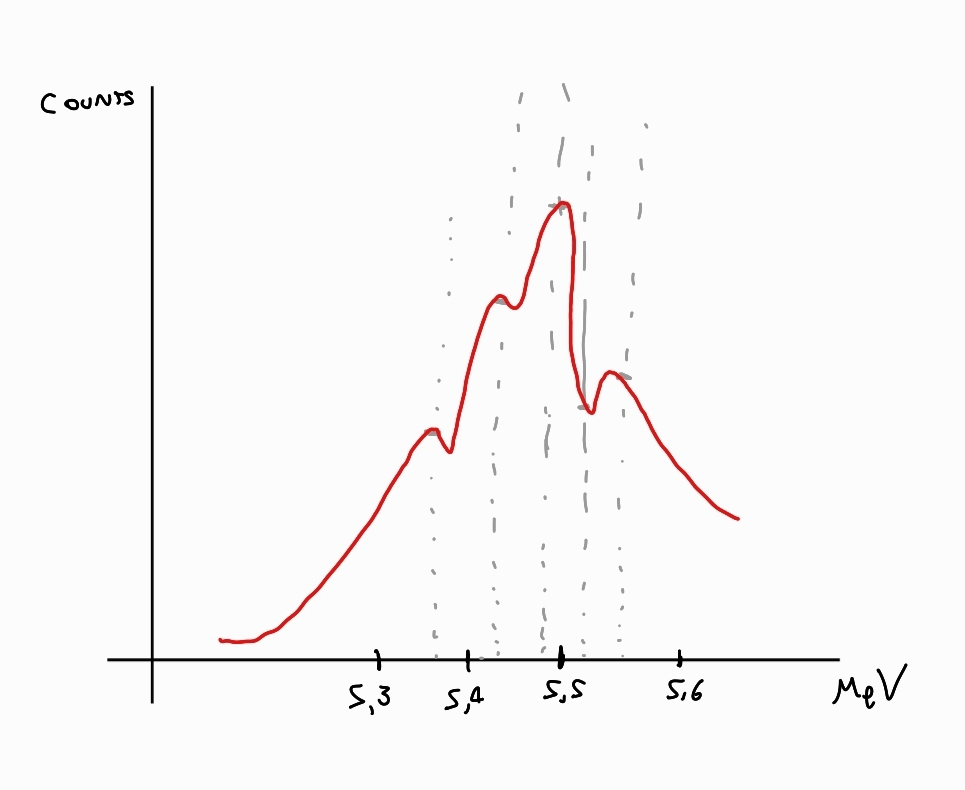
\includegraphics[width=0.7\linewidth]{imagenes/tempFileForShare_20240411-123131}
		\caption{Espectro de radiación de Am$^{241}$ dibujado}
		\label{fig:dibujo}
	\end{figure}
	
	
	\begin{table}[H]
		\centering
		\begin{tabular}{|c|c|c|}
			\hline
			Distancia (cm) & Cuentas & Bq   \\ \hline
			1              & 42343   & 143  \\ \hline
			1,5            & 8485    & 28,3 \\ \hline
			2              & 5924    & 19,8 \\ \hline
			2,5            & 3584    & 12   \\ \hline
			3              & 2607    & 8,7  \\ \hline
			3,5            & 1102    & 3,67 \\ \hline
		\end{tabular}
	\caption{Radiación $\alpha$ según distancia}
	\end{table}
	
	
	
	
\begin{figure}[H]
	\centering
	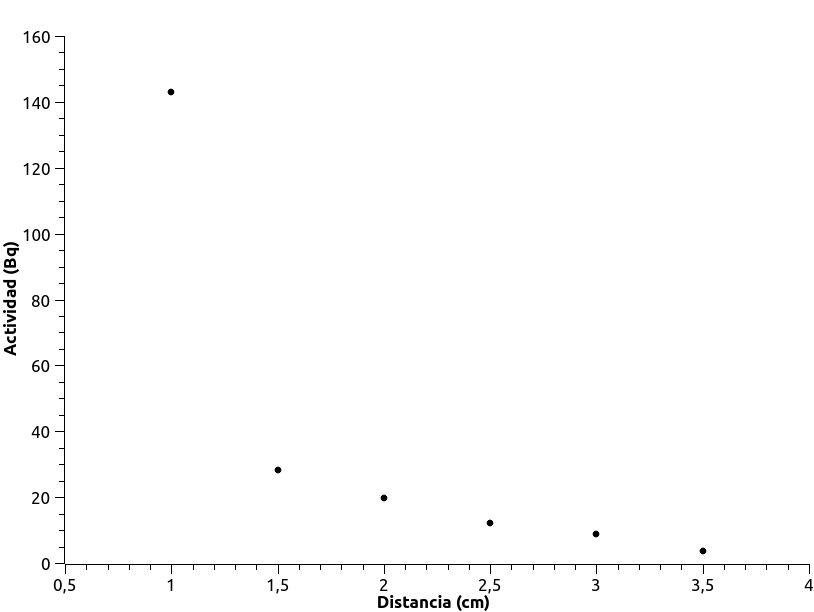
\includegraphics[width=0.9\linewidth]{imagenes/5_1}
	\caption[Actividad $\alpha$ según distancia]{}
	\label{fig:51}
\end{figure}
	
	
	Vemos que el alcance de las partículas $\alpha$ es muy pequeña, y que su energía se reduce considerablemente por la cantidad de interacciones con electrones. Los electrones no son muchos, pero las partículas $\alpha$ son muy másicas.\\
	
	
	
	Al colocar el filtro de celofán, la radiación se bloquea por completo, no llega nada al detector.
	Las partículas $\alpha$ interactúan fuertemente con la materia a través de la ionización, e incluso el celofán tiene una densidad suficiente para bloquear esta fuente.\\
	
	
	En definitiva, por el bajo alcance y penetración que tienen las partículas $\alpha$, podemos decir que la protección que requieren los humanos se puede limitar a no introducir emisores en su organismo, ya que la radiación no llega muy lejos, y en caso de llegar es bloqueada por la piel.
	
	
	\section{Eficiencia del detector para $\alpha$}
	
	Utilizamos el área del espectro para la menor distancia, y lo dividimos entre el tiempo para obtener la actividad experimental.
	
	\[A' = \frac{\text{Cuentas}}{t}= \frac{52343}{300} = 141,143 \si{Bq}\]
	
	Calculamos la actividad corregida de la muestra, conociendo que en 2019 presentaba una actividad inicial de 3,7KBq (este cálculo lo realizamos en 2024, 5 años de diferencia).
	
	\[T_{1/2}= 458 \text{años}\]
	\[A = A_0 \text{e}^{-\frac{\ln 2}{T_{1/2} } t} = 3,672 \si{KBq}\]

	
	
	\[\varepsilon = \frac{A'}{A} = \frac{141,143\si{Bq}}{367,2 \si{Bq} }= 0,0384  \longrightarrow \varepsilon =  3,84\%
	\]
	
	 \vspace{\baselineskip}
	
	\section{Espectro $\beta$ del Sr$^{90}$}
	
	Introducimos la muestra de Sr$^{90}$ en el detector y acumulamos hasta obtener una buena estadística.
	
	La Figura \ref{fig:17} es el espectro obtenido
	
	
\begin{figure}[H]
	\centering
	\includegraphics[width=0.7\linewidth]{"graficas recortadas/17"}
	\caption{Espectro del Sr$^{90}$}
	\label{fig:17}
\end{figure}
	
	Se trata de una distribución contínua, por lo que las partículas beta pueden tener una amplia gama de energías, desde el mínimo hasta un máximo determinado por la energía liberada en el proceso de desintegración.
	La forma de este espectro se debe a la superposición de la radiación de las dos desintegraciones que tienen lugar en el Estroncio-90, que podemos ver en la Figura \ref{fig:desintsr90}. 
	
\begin{figure}[H]
	\centering
	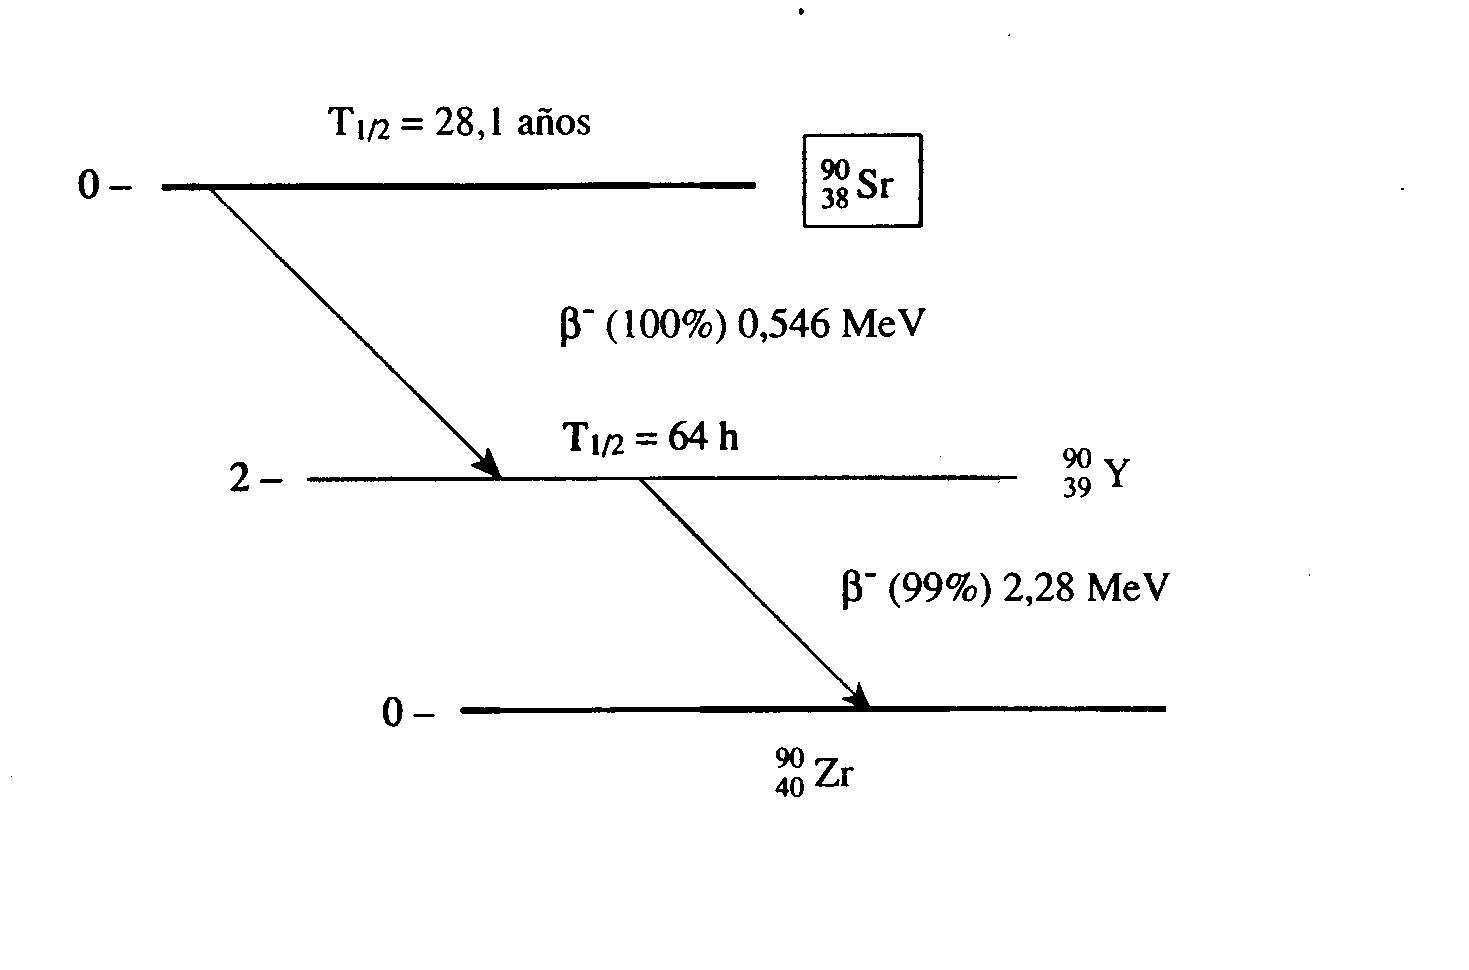
\includegraphics[width=0.7\linewidth]{imagenes/image.C52AM2}
	\caption{Esquema de desintegración del Sr$^{90}$}
	\label{fig:desintsr90}
\end{figure}

	La primera tiene una energía máxima de 0,546MeV, y la segunda llega hasta 2,28MeV. Dado que están superpuestas, el número de cuentas a bajas energías es alto.
	
	


	\section{Calibración en energías para $\beta$}
	
	
	Calibramos la medida, estableciendo la energía máxima en el límite derecho. \\
	
	Midiendo el area bajo el espectro obtenemos 157842 cuentas, que como han sido obtenidas en 899s, equivale a una actividad de 175,58Bq.
	
	\subsection*{Eficiencia en $\beta$}
	
	La muestra utilizada tiene una actividad inicial de 0,1$\mu$Ci en enero de 2020 (hace 4,17 años). Por tanto su actividad corregida:
	
	\[A = A_0 \text{e}^{-\frac{\ln 2}{T_{1/2} t}}\]
	\[T_{1/2}= 28,1\text{años}\]
	\[t = 4,17 \text{años}\]
	
	\[A = 0,09\si{\mu Ci} = 3338,58 \si{Bq}\]
	
	La eficiencia por tanto:
	\[ \varepsilon = \frac{A'}{A} = \frac{175,58\si{Bq}}{ 3338,58 \si{Bq}} = 0,0526 
	\]
	\[\varepsilon = 5,26\%
	\]
	
	En la primera práctica vimos la eficiencia de un detector Geiger para este mismo emisor, Estroncio-90, y vimos que daba 7,65\%. El detector Geiger es más eficiente detectando partículas $\beta$ de alta energía, ya que aunque los detectores de barrera de superficie pueden ser útiles para detectar partículas de baja energía, la profundidad de penetración de las partículas de alta energía hace que puedan atravesar el semiconductor sin depositar toda su energía, reduciendo la eficiencia.
	
	
	
	
	%[Para calibrar se utiliza el espectro del Sr 90 . Se toma el límite izquierdo como energía cero y donde acaba el espectro como la energía máxima del β del Y-90, que aparece en el esquema de desintegración.]
	
	%Compruebe la calibración, para ello mire dónde estaría la energía máxima del β del Sr 90 . Dibújelo en el espectro.
	
	%Determine la eciencia del detector para las betas.
	
	\section{Absorción en plomo}
	
\begin{figure}[H]
	\centering
	\includegraphics[width=0.7\linewidth]{"graficas recortadas/18"}
	\caption{Espectro del Sr$^{90}$ al colocar el filtro de plomo}
	\label{fig:18}
\end{figure}
	
	A simple vista podemos ver que cantidad de radiación se ha reducido debido a la interacción de las partículas con el plomo, pero sigue presentando la misma distribución de energías.\\
	
	La cantidad de radiación medida es de 8330 cuentas, que a 504s corresponden con una actividad percibida de 16,53Bq.\\
	
	Actividad sin plomo: 157842 cuentas
	Actividad con plomo: 8330 cuentas
	
	La reducción de la actividad ha sido de 
	\[ \frac{8330}{157842} = 0,053 \longrightarrow 5,3\%
	\]
	
	Por lo tanto el filtro de plomo está frenando un 95\% de la radiación $\beta$.   
	
	\section{Estudio de la conversión interna}
	
	Insertamos una muestra de Cesio-137 y obtenemos su espectro de radiación $\beta$.
	
	
	\begin{figure}[H]
		\centering
		\includegraphics[width=0.7\linewidth]{"graficas recortadas/19"}
		\caption{Espectro $\beta$ del Cs$^{137}$}
		\label{fig:19}
	\end{figure}
	
	El espectro presenta una forma contínua con dos picos. El pico de la izquierda se produce por la desintegración $\beta^{-}$ del cesio, a 0,512MeV. \\
	
	El segundo pico se produce por la conversión interna de gammas y betas, que se produce a 1,17MeV.
	
	Este efecto se produce cuando un átomo experimenta una transición electrónica en la que un electrón es expulsado de una capa interna y es reemplazado por un electrón de una capa superior. El proceso resulta en la emisión de un fotón de rayos X cuya energía es igual a la diferencia entre las energías de los dos niveles de electrones involucrados en la transición.
	
	
	
	
	
	
\end{document}






